\documentclass{article}

\usepackage{arxiv}

\usepackage[utf8]{inputenc} % allow utf-8 input
\usepackage[T1]{fontenc}    % use 8-bit T1 fonts
\usepackage{hyperref}       % hyperlinks
\usepackage{url}            % simple URL typesetting
\usepackage{booktabs}       % professional-quality tables
\usepackage{amsfonts}       % blackboard math symbols
\usepackage{nicefrac}       % compact symbols for 1/2, etc.
\usepackage{microtype}      % microtypography
\usepackage{graphicx}
\usepackage{natbib}
\usepackage{doi}

\usepackage{amsmath}
\usepackage{nicematrix}
\usepackage{cleveref}
\usepackage{listings}
\usepackage{pgfplots}

\usepackage{algpseudocode}
\usepackage{algorithm}

\hypersetup{
    colorlinks=true,
    linkcolor=blue,
    filecolor=magenta,
    urlcolor=blue,
    pdftitle={Overleaf Example},
    pdfpagemode=FullScreen,
    }

\renewcommand{\algorithmicrequire}{\textbf{Input:}}
\renewcommand{\algorithmicensure}{\textbf{Initialize:}}

\NiceMatrixOptions{cell-space-top-limit=5pt,cell-space-bottom-limit=5pt,columns-width=20pt}

\Crefname{lstlisting}{listing}{listings}
\Crefname{lstlisting}{Listing}{Listings}


% Listing options
\definecolor{codegreen}{rgb}{0,0.6,0}
\definecolor{codegray}{rgb}{0.5,0.5,0.5}
\definecolor{codepurple}{rgb}{0.58,0,0.82}
\definecolor{backcolour}{rgb}{0.95,0.95,0.92}

\lstdefinestyle{python_style}{
    backgroundcolor=\color{backcolour},
    commentstyle=\color{codegreen},
    keywordstyle=\color{magenta},
    numberstyle=\tiny\color{codegray},
    stringstyle=\color{codepurple},
    basicstyle=\ttfamily\footnotesize,
    breakatwhitespace=false,
    breaklines=true,
    captionpos=b,
    keepspaces=true,
    numbers=left,
    numbersep=5pt,
    showspaces=false,
    showstringspaces=false,
    showtabs=false,
    tabsize=2
}
\lstset{style=python_style}
\NewDocumentCommand{\codeword}{v}{%
\texttt{\textcolor{blue}{#1}}%
}

\def\R{\mathbb{R}}


\title{EBREG-RL: Example-Based Regular Expression Generator
via Reinforcement Learning}

%\date{September 9, 1985}	% Here you can change the date presented in the paper title
\date{} 					% Or removing it

\author{
  \hspace{1mm}Dmitry Beresnev\\
	AIDS-MS1, Innopolis University\\
	\texttt{d.beresnev@innopolis.university}\\
	\And{}
  \hspace{1mm}Vsevolod Klyushev\\
	AIDS-MS1, Innopolis University\\
	\texttt{v.klyushev@innopolis.university}	\And{}
  \hspace{1mm}Nikita Yaneev\\
	AIDS-MS1, Innopolis University\\
	\texttt{n.yaneev@innopolis.university}
}

\renewcommand{\undertitle}{Project report for RL\&IA course S25 Innopolis University}
\renewcommand{\headeright}{}

\pgfplotsset{compat=1.18}
\begin{document}
\maketitle


\section{Introduction}

Nowadays Big-Tech companies increasingly prefer data-driven development, which requires careful extraction of
information, including from unstructured or almost unstructured text. This task is considered as extremely tough,
but in many real-world scenarios even unstructured text information have underlying syntactic pattern that can be
characterized by a regular expressions, due to their adaptability and expressiveness.
However, even for experienced programmers, writing RegEx by hand is a boring, time-consuming, and error-prone
process. Moreover, despite widespread use of regular expression, there are not so many researches and literature on
the automatic RegEx generation. That is why we have chosen an example-based RegEx generation as a topic of the project of
this course.

\begin{figure}[H]
  \centering
  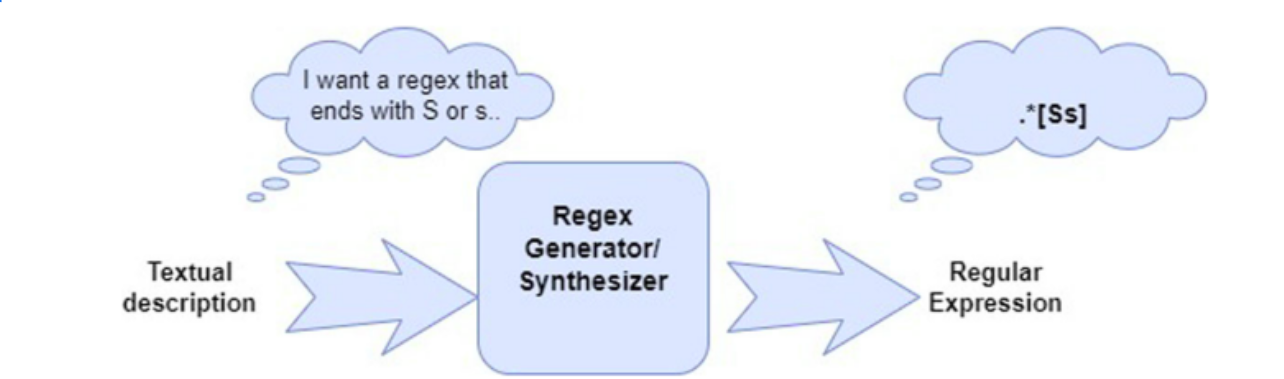
\includegraphics[width=0.6\textwidth]{./pictures/approach1.png}
  \caption{Natural Language to Regex (NL2RE) pipeline}\label{fig:NL2RE}
\end{figure}

One approach~\cite{Zhong2018, Tariq2024} uses LLMs to convert natural language prompts into regular expressions \Cref{fig:NL2RE}.
This method offers flexibility, allowing the model to generate a wide variety of RegExes.
However, it requires significant computational resources and careful architecture design.
This method is not ideal for generating RegExes that are specifically tailored to a particular domain or task.
It is also challenging to ensure that the generated RegExes are accurate and efficient.

Another approach~\cite{Bartoli2016, Bartoli2018} uses genetic programming (GP) to generate regular expression for specific tasks based on labeled
data. The GP algorithm searches for the best-performing regular expression by iteratively evolving a population of
candidate solutions. This method requires careful design of hyper-parameters, such as the size of the population and
the mutation rate, as well as a well-defined fitness function to evaluate the performance of each regular expression.

\section{Problem formulation}

We propose a new approach that leverages reinforcement learning (RL) to generate regular expression.
This method formulates the regular expression generation process as a Markov decision process (MDP)
with fully-observable deterministic episodic environment.

Each action corresponds to a regular expression syntax unit, state space would be a set of all possible sequences
of syntax units of fixed length.

\subsection{Reverse Polish Notation}
Due to the fact that regular expressions have operations with different precedence and number of arguments,
we decided to use the Reverse Polish Notation (RPN) for the construction of regular expressions.

In our Regex RPN implementation we have 103 different tokens:
\begin{itemize}
  \item 92 simple tokens (letters, digits, quantifiers, and symbols, etc.),
  \item 2 binary operations (\codeword{concat} and \codeword{|}),
  \item 6 unary operations (\codeword{*}, \codeword{+}, \codeword{?}, \codeword{*?}, \codeword{+?}, \codeword{??}),
  \item 3 many to one operations (\codeword{[]}, \codeword{^[]}, \codeword{concat_all}).
\end{itemize}

Let us demonstrate, how RPN representation is converted to the infix (regular) notation. Suppose the following list of tokens as input to RPN: [\codeword{1}, \codeword{a}, \codeword{b}, \codeword{[]}, \codeword{*}]
By iterating one after another, the following (infix) expressions would be generated:

\begin{enumerate}
  \item \codeword{1}
  \item \codeword{a1}
  \item \codeword{ba1}
  \item \codeword{[ba1]}
  \item \codeword{[ba1]*}
\end{enumerate}

Another example with the RPN {[\codeword{\d}, \codeword{@}, \codeword{|}, \codeword{[]}, \codeword{+} ]}
\begin{enumerate}
  \item \codeword{\d}
  \item \codeword{@\d}
  \item \codeword{\d|@}
  \item \codeword{[\d|@]}
  \item \codeword{[\d|@]+}
\end{enumerate}

You can find more about RPN \href{https://en.wikipedia.org/wiki/Reverse_Polish_notation}{here}.


\subsection{Dataset}

We have decided to construct the dataset (given true regular expression) in the following form:
\begin{itemize}
  \item Text
  \item Nonempty list of indexes (begin and end) of symbols from example text, which we want to retrieve with achieved regex
\end{itemize}

\section{Methodology}
This section explains the underlying RL theory and solution design aspects.
\subsection{Action Space}
Action space for our RL agent consists of all possible RPN tokens together with \codeword{FIN} state (to finish regex construction earlier). In total we have 104 actions in our action space.

\subsection{State Space}
The state space $s$ consists of $n$ placeholders, where each placeholder can either contain an action
from the action space or remain empty (denoted by a special empty token). After the agent
takes an action at step $i$ (say we count from 0, so the first step is at $i=0$) $a_i$, the state
is updated as $s_i \gets a_i$.

\subsection{Reward}
The reward in the considered task is delayed and is calculated in the final state (if the action is \codeword{FIN} or the maximum length of regex is achieved). The rewards on each non-terminate state is 0.
We come up with two approaches for reward calculation.
Let's start with common parts.

Firstly, we start with a text from which we want to extract specific information. To do this, we need to construct a `target bit-mask' of length $n$ (where $n$ is the text length), where:
\begin{itemize}
  \item 1 marks positions to be included
  \item 0 marks positions to be excluded
\end{itemize}

Then, we create the `found' regular expression from the terminate state form RPN and apply it to the text, retrieving indices of found symbol.
After that, we construct the `current bit-mask' in the same way as `target bit-mask'.


\subsubsection{Xor approach}
First idea of the reward was the following:
\begin{equation}
  R = a \cdot \sum(A \oplus B) + b \cdot |C - D| + c \cdot E
\end{equation}
where:
\begin{itemize}
  \item $A$ --- `target bit-mask'
  \item $B$ --- `current bit-mask'
  \item $C$ --- number of target words
  \item $D$ --- number of words, retrieved with regex
  \item $E$ --- token length of regex
\end{itemize}

Our final parameters for the environment that were the most successful are as follows
\begin{itemize}
  \item Index mismatch $a = -100$
  \item Mismatch in words $b = -10000$
  \item Penalty for length $c = -1$
\end{itemize}
\subsubsection{Metrics approach}
Second idea of the reward is based on the fact, that we can calculate accuracy and F1 on bit-masks.
Thus reward function would be the following:
\begin{equation}
  R =a \cdot (\text{F1} -1) + b \cdot (A-1) + c \cdot \sum(A \oplus B) + d \cdot |C - D| + e \cdot E\
\end{equation}

where:
\begin{itemize}
  \item F1 --- F1 score on bit masks
  \item $A$ --- Accuracy on bit masks
  \item $C$ --- number of target words
  \item $D$ --- number of words, retrieved with regex
  \item $E$ --- token length of regex
\end{itemize}

Our final parameters for the environment that were the most successful are as follows
\begin{itemize}
  \item The weight of the F1 metric $a = 100$
  \item The weight of the Accuracy metric $b = 100$
  \item Index mismatch $c = 100$
  \item Mismatch in words $d = -1$
  \item Penalty for length $e = -0.1$

\end{itemize}


\section{Reinforcement Learning algorithms}
We decided to check three RL algorithms: Advantage Actor-Critic (A2C), REINFORCE and Deep Q-Network (DQN).

\subsection{REINFORCE}
REINFORCE is a version of Monte-Carlo Policy Gradient algorithm proposed by
Williams in~\cite{Williams1992}. It adopts an explicit stochastic policy, and
uses the episode samples to update the policy parameters. To construct the
sample space, the full episode should be played, which correlates with the
proposed solution architecture.

\paragraph{Policy}
In the case of using REINFORCE, the stochastic policy of selection action $a_t$
given state $s_t$ obtained from policy:
\begin{align}
  \label{eq:rnf_policy}
  \pi_{\theta}(a_t | s_t) =
  \operatorname{softmax}(\text{MLP}(\theta)),
\end{align}
where $\theta$ denotes the parameters of policy neural network.

During training stage, the corresponding probabilities from
\Cref{eq:rnf_policy} are used for action sampling. During evaluation and
testing stages, the optimal action $a_t^\ast$ is chosen in the following way:
\begin{align}
  \label{eq:rnf_optimal}
  a_t^\ast = \operatorname{argmax}_{a}\pi_{\theta}(a | s_t)
\end{align}

\paragraph{Objective function}
The expected reward definition is manly based on one given in~\cite{Zhang2018}.

The main goal of policy optimization is maximizing the expected reward, which
is defined as
\begin{multline}\label{eq:rnf_expreward}
  J(\theta) = \mathbb{E}_{(s_t, a_t) \sim P_{\theta}(s_t, a_t)} r(s_1 a_1 \dots s_N
  a_N) = \sum_{s_1 a_1 \dots s_N a_N} P_{\theta}(s_1 a_1 \dots s_N a_N)R_N \\ =
  \sum_{s_1 a_1 \dots s_N a_N} p(s_1) \prod_t \pi_{\theta}(a_t | s_t)p(s_{t+1}|
  s_t, a_t)R_N.
\end{multline}
Here for the simplicity it is assumed,
that $N$ --- total length of episode.
By the solution architecture design, the state $s_{t+1}$ is completely
determined by state $s_t$ and action $a_t$, the probabilities
$p(s_1)$ and $p(s_{t+1}|s_t, a_t)$ are both equal to 1. Therefore,
the \Cref{eq:rnf_expreward} can be simplified to
\begin{align}
  J(\theta) = \sum_{s_1 a_1 \dots s_N a_N}\prod_t \pi_{\theta}(a_t | s_t)R_N.
\end{align}

The likelihood ratios are then used to compute the policy gradient:
\begin{align}
  \label{eq:rnf_pg}
  \nabla_{\theta} J(\theta) = R_N \sum_{t=1}^N \nabla_{\theta} \log \pi_{\theta}(a_t | s_t).
\end{align}

In addition to just policy gradient, the entropy $H$ of the policy is included
to the objective function. Entropy is defined as
\begin{align}
  \label{eq:entropy}
  H(\theta) = - \sum_a \pi_{\theta}(a | s) \log \pi_{\theta}(a | s).
\end{align}
The value of $H$ is always non-negative, and has a single maximum
when all the actions have the same probability to be taken, i.e.\ when
policy is uniform. Entropy reaches minimum, when
$\pi_{\theta}(a_i | s) = 1$ for some action $a_i$ and
$\pi_{\theta}(a_j | s) = 0$ for all $j \neq i$. Therefore,
subtracting the entropy from the objective function pushes the policy to be uniform,
what means punishing the agent to be too sure about what action to take.

Finally, the objective function for the policy update combines
\Cref{eq:rnf_pg,eq:entropy}, and is defined as
\begin{align}
  \label{eq:rnf_objective}
  Z(\theta) = \nabla_\theta J(\theta) - \beta \nabla_\theta H(\theta),
\end{align}
where $\beta$ is hyperparameter to balance two terms, which is usually
called \textit{entropy beta}.

\subsection{Advantage Actor-Critic (A2C)}\label{subsubsec:a2c}

The Actor-Critic method combines the policy-based and value-based approaches.
In this method, two function approximations are learned: policy function
$\pi_{\theta}(a|s)$, which controls what action the agent selects at state $s$,
and value function $v_{\theta}(s)$, which estimates how profitable the state
$s$ is.

The modification of Actor-Critic method, which uses advantage, is called
Advantage Actor-Critic (A2C) and is used for more stable convergence in
comparison with only policy-based methods, like REINFORCE. The advantage is
calculated in the following way:
\begin{align*}
  A(s_t, a_t) = q(s_t,a_t)- v(s_t),
\end{align*}
where $ q(s_t,a_t)$ --- action value function.

\begin{align}\label{eq:q_estimation}
  q(s,a) \approx R_N = \sum_{t=1}^N \gamma^{N-t}_\text{decay} r_t.
\end{align}
where $\gamma_\text{decay}$ --- decay factor, which is between 0 and 1,
and $r_t$ is the reward at state $s_t$ and total episode return $R_N$.

Advantage $A(s_t, a_t)$ indicates the extra reward the agent can get if it
selects the action $a_t$ at state $s_t$ compared to the mean reward, $v(s_t)$,
it gets at state $s_t$. Using the \Cref{eq:q_estimation}, the formula for
advantage becomes the following:
\begin{align}
  \label{eq:a2c_advantage}
  A(s_t, a_t) = R_N - v(s_t).
\end{align}

\begin{figure}[hbt]
  \centering
  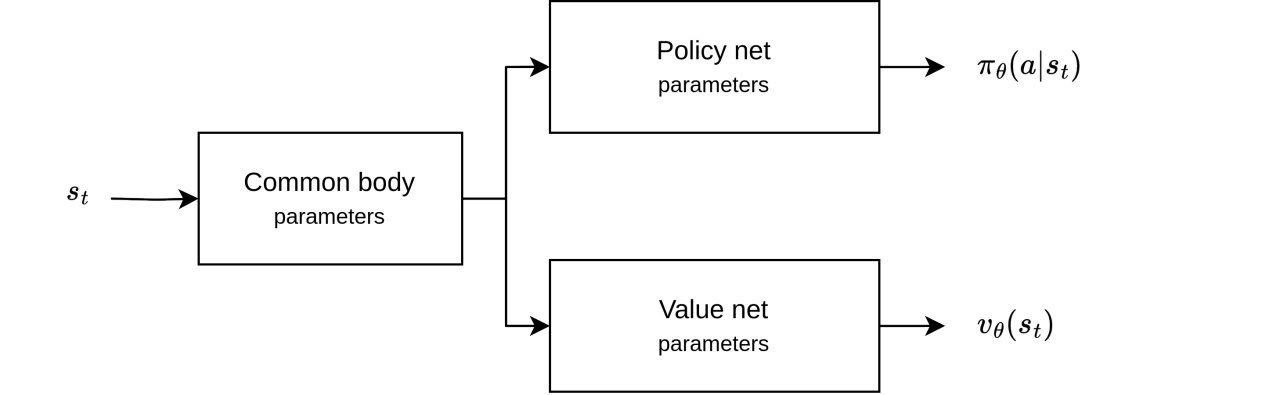
\includegraphics[width=\textwidth,keepaspectratio]{pictures/a2c.jpg}
  \caption[Advantage Actor-Critic (A2C) architecture with shared body]
  {Advantage Actor-Critic (A2C) architecture with shared body.
  }\label{fig:a2c_arch}
\end{figure}

\paragraph{Policy}
The policy calculation is similar to REINFORCE case (\Cref{eq:rnf_policy}). The
stochastic policy of selection action $a_t$ given state $s_t$ obtained from
policy head of neural network depicted on \Cref{fig:a2c_arch}.

During training stage, the corresponding probabilities $\pi_{\theta}(a_t | s_t)$
are used for action sampling. During evaluation and
testing stages, the optimal action $a_t^\ast$ is chosen in the same way as in
\Cref{eq:rnf_optimal}.

\paragraph{Objective function}
At the beginning, it is necessary to define $v_\theta(s_t)$. The value function
of the given state $s_t$ obtained from value head of neural network depicted on \Cref{fig:a2c_arch}.

The objective function itself in case of A2C consists of three parts: policy
gradient part, entropy part and value loss part.

First part is policy gradient, which is quite similar to the one give in
\Cref{eq:rnf_pg}:
\begin{align*}
  \nabla_{\theta} J(\theta) =
  \sum_{t=1}^N A(s_t, a_t)\nabla_{\theta}  \log \pi_{\theta}(a_t | s_t).
\end{align*}
The only difference is that, instead of $q_\theta(s_t, a_t)$ used
\Cref{eq:rnf_pg},
here $A(s_t, a_t)$ is used. Using the \Cref{eq:a2c_advantage},
the policy gradient formula becomes as following:
\begin{align}
  \label{eq:a2c_pg}
  \nabla_{\theta} J(\theta) =
  \sum_{t=1}^N (R_N - v_\theta(s_t)) \nabla_{\theta} \log \pi_{\theta}(a_t | s_t).
\end{align}

Second part of objective function is entropy part, $H(\theta)$, which is
identical to one proposed for REINFORCE (\Cref{eq:entropy}).

Third and final part of objective function is value loss part, which estimates
how accurate net approximates value. The value loss is defined as
\begin{align}
  \label{eq:a2c_vl}
  L_v(\theta)
  =\sum^N_{t=1} {(q_{\theta}(s_t, a_t) - v_{\theta}(s_t))}^2
  = \sum^N_{t=1} {(R_N- v_\theta(s_t))}^2.
\end{align}

The objective function is defined as the following combination of
\Cref{eq:a2c_pg,eq:entropy,eq:a2c_vl}:
\begin{align}
  \label{eq:a2c_objective}
  Z(\theta) = \nabla_\theta J(\theta) +
  \nabla_\theta L_v(\theta) - \beta \nabla_\theta H(\theta),
\end{align}
where $\beta$ has the same meaning as in \Cref{eq:rnf_objective}.


\subsection{Deep Q-Network (DQN)}\label{subsubsec:dqn}

The Deep Q-Network (DQN) approximates a state-value function $Q(s, a)$ for each
possible action and state, using the experience replay buffer. Therefore, the
DQN policy, which is build based on the state-value function, is implicit and
deterministic.

Q-Network is usually optimized towards target network with frozen weights,
which is denoted as $\hat{Q}(s, a)$. In its turn, the target network is
periodically updated with the latest Q-Network weights every $k_\text{sync}$
episodes, where $k_\text{sync}$ is a hyperparameter. The target network is
introduced to stabilize training.

\paragraph{Policy}
To perform agent exploration, the $\epsilon$-greedy strategy is used.
$\epsilon(i)$ is a function $\mathbb{R}^d \rightarrow (0, 1)$, which maps the
index of current epoch to float value between 0 and 1. On each step, the agent
with the probability of $\epsilon$ selects random action. Otherwise, the agent
selects action which maximizes $Q(s, a)$. This can be formalized as follows:
\begin{align}
  \label{eq:dqn_policy}
  \pi_{\theta}(s_t) =
  \begin{cases}
    a \sim \{a_m\}                          & \text{ with probability } \epsilon,     \\
    \operatorname{argmax}_a Q_\theta(s_t,a) & \text{ with probability } 1 - \epsilon.
  \end{cases}
\end{align}
where $\theta$
denotes the parameters of neural network and
$\{a_m\}$ --- actions space.

During training stage, the actions are sampled according to the
\Cref{eq:dqn_policy}. During evaluation and testing stages, the optimal action
$a_t^\ast$ is chosen as $a_t^\ast =\text{argmax}_a Q_\theta(s_t,a)$.

\paragraph{Objective function}
In case of DQN, the objective function for the episode consists only form one
part --- state-value loss $L_Q(\theta) = \sum_{t=1}^N L_{Q_t}(\theta)$, and
$L_{Q_t}(\theta)$ is defined as following:
\begin{align*}
  % \label{eq:dqn_objective}
  L_{Q_t}(\theta) =
  \begin{cases}
    {(Q_\theta(s_t,a) - R_N)}^2,                                         & \text{ if the episode has ended} \\
    {(Q_\theta(s_t,a) - \max_{a'}\hat{Q}_{\hat{\theta}}(s_{t+1},a'))}^2, & \text{ otherwise}.
  \end{cases}
\end{align*}
Note that for non-terminal states the target network
$\hat{Q}(s,a)$ is used to predict value of the next state $s_{t+1}$.
Also recall that every $k_\text{sync}$ episodes $\hat{\theta}$ is set
to $\theta$.

Therefore, the objective function looks like the following:
\begin{align}
  \label{eq:dqn_objective}
  Z(\theta) = \nabla_\theta L_Q(\theta).
\end{align}




\section{Experiments}
We have decided to check our models on three different experiments:
extraction of single number (low complexity), extraction of word consisting of
specified set of symbols (medium complexity) and extraction ef email (high complexity).
Each experiment has corresponding dataset.

Note that in experiments DQN approach is not presented as it demonstrates pure
performance on toy tasks during development. The main reason is that DQN is value-based approach
(while REINFORCE and A2C are policy-based) what means the exploration-exploitation
trade-off should be explicitly defined. However, we fails to find the good $epsilon$-greedy
strategy: either agent explored too much and failed to converge, or agent started exploiting too
early and failed to explore all actions.  Therefore, we decided to abandon DQN and switch to algorithms that update the policy directly.

\subsection{Single number retrieval}
The task is to retrieve single number from the string of characters. Number is defined as one or more digit.

\begin{figure}[H]
  \centering
  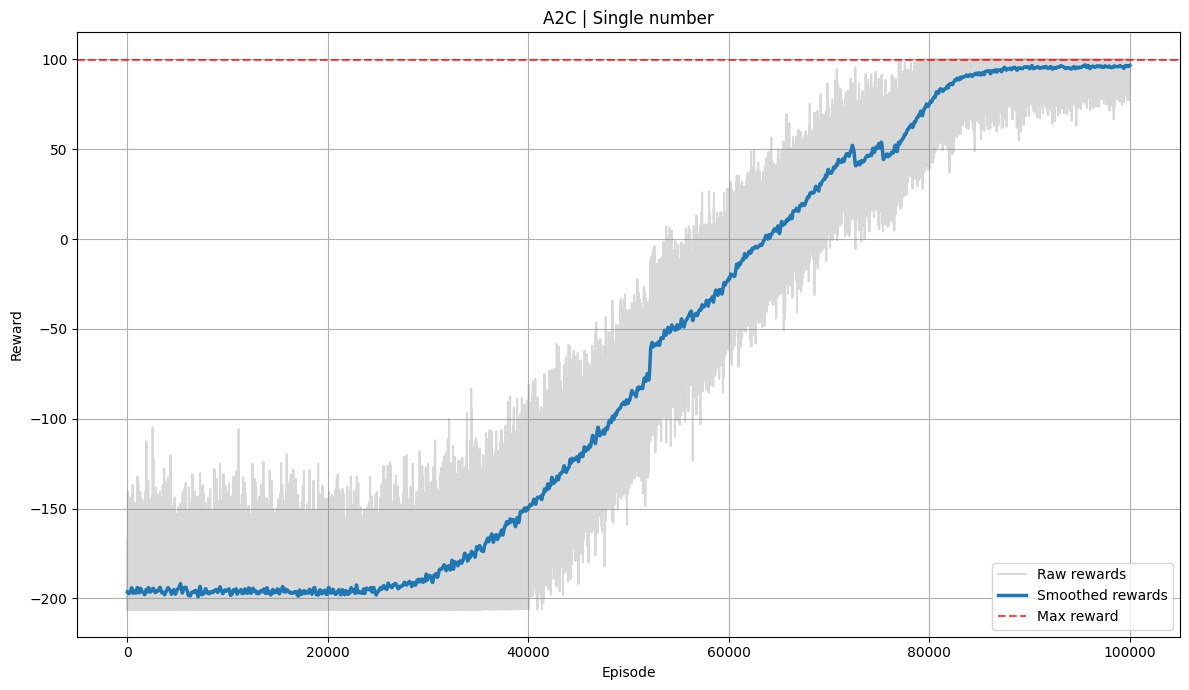
\includegraphics[width=0.7\textwidth]{./pictures/a2c_number.jpg}
  \caption[A2C convergence on Single Number Retrieval problem]
  {A2C convergence on Single Number Retrieval problem}\label{fig:a2c_num}
\end{figure}

\begin{figure}[H]
  \centering
  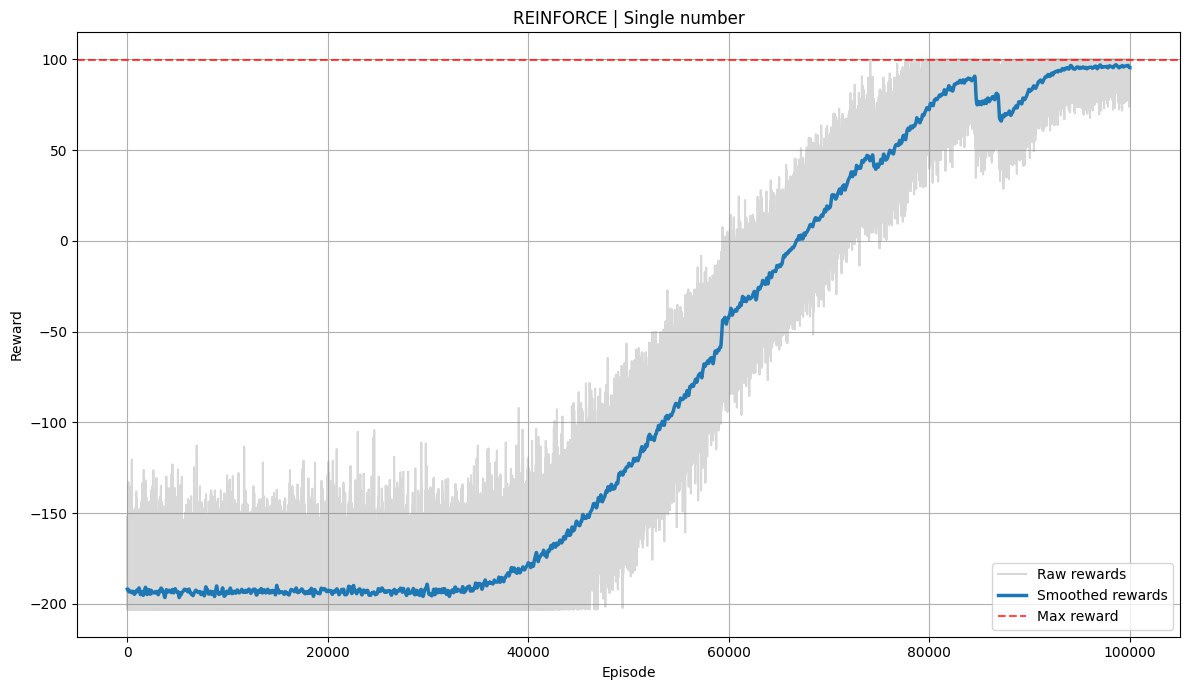
\includegraphics[width=0.7\textwidth]{./pictures/reinforce_number.jpg}
  \caption[REINFORCE convergence on Single Number Retrieval problem]
  {REINFORCE convergence on Single Number Retrieval problem}\label{fig:reinforce_num}
\end{figure}

\begin{figure}[H]
  \centering
  \begin{tabular}{l|l|l}
    \toprule
    \textbf{Agent} & \textbf{Achieved Regex} & \textbf{Total Reward} \\
    \midrule
    A2C            & \codeword{\d+}          & 49899.99              \\
    REINFORCE      & \codeword{\d+}          & 49899.99              \\
    Random agent   & \codeword{v1\+.r}       & -66791.97             \\
    \bottomrule
  \end{tabular}
  \caption{Final results for Single Number Retrieval problem. \textit{Total Reward} is the sum of rewards on all dataset samples}\label{tab:res_num}
\end{figure}


\paragraph{Dataset}
The dataset contains 500 strings of lengths from 3 to 10. Each string includes one number (maximum 3 digits).

\paragraph{Target regex}
We want our RL agent to simulate the application of \codeword{\d} regular expression.

\paragraph{Results}
\Cref{fig:a2c_num,fig:reinforce_num} show that both algorithms converged to the quite high positive rewards. \Cref{tab:res_num} demonstrates that obtained regular expressions are indeed correct.

\subsection{Word from subset of symbols retrieval}
The task is to retrieve a word which consists of a certain subset of symbols from the string.
Word is a string with one or more symbols.


\begin{figure}[H]
  \centering
  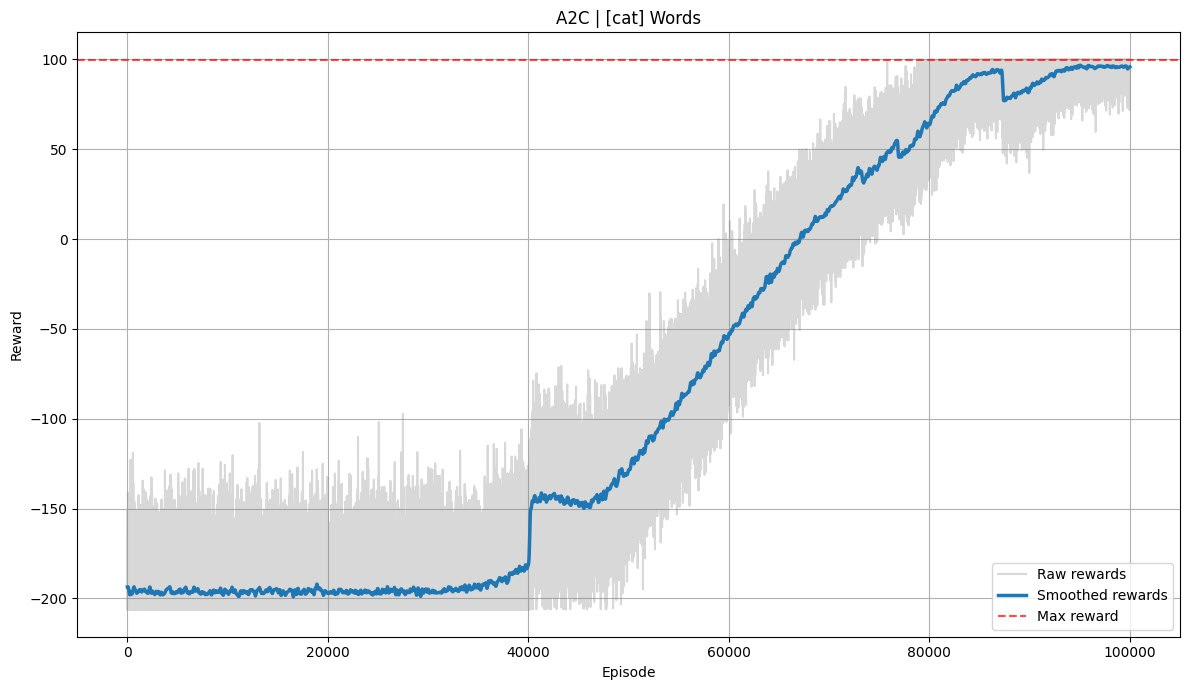
\includegraphics[width=0.7\textwidth]{./pictures/a2c_words.jpg}
  \caption[A2C convergence on Single Number Retrieval problem]
  {A2C convergence on Word Retrieval problem}\label{fig:a2c_word}
\end{figure}

\begin{figure}[H]
  \centering
  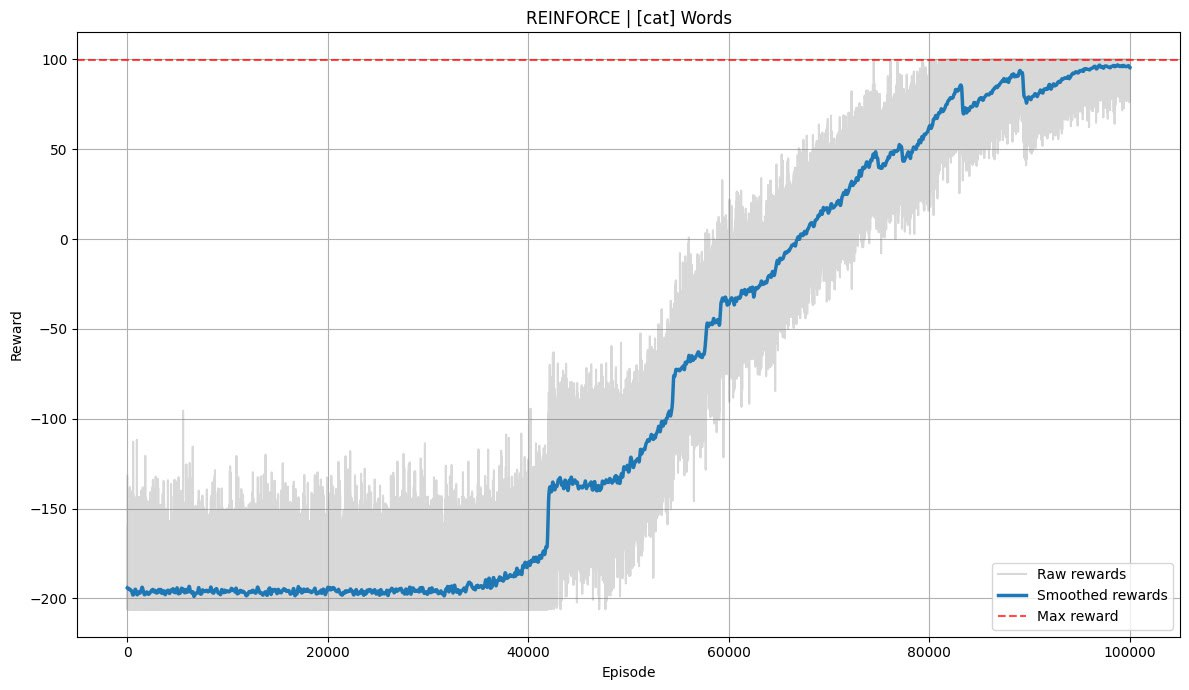
\includegraphics[width=0.7\textwidth]{./pictures/reinforce_words.jpg}
  \caption[REINFORCE convergence on Word Retrieval problem]
  {REINFORCE convergence on Word Retrieval problem}\label{fig:reinforce_word}
\end{figure}

\begin{figure}[H]
  \centering
  \begin{tabular}{l|l|l}
    \toprule
    \textbf{Agent} & \textbf{Achieved Regex} & \textbf{Total Reward} \\
    \midrule
    A2C            & \codeword{[atc]+}       & 49749.99              \\
    REINFORCE      & \codeword{[tca]+}       & 49749.99              \\
    Random agent   & \codeword{7CbQr}        & -65763.80             \\
    \bottomrule
  \end{tabular}
  \caption{Final results for Word Retrieval problem. \textit{Total Reward} is the sum of rewards on all dataset samples}\label{tab:res_word}
\end{figure}


\paragraph{Dataset}
The dataset contains 500 strings of lengths from 6 to 20. Each string includes one word that consists of the letters `c', `a' and `t'.

\paragraph{Target regex}
We want our RL agent to simulate the application of \codeword{[cat]+} regular expression.
Note that actually every combination of letters `c', `a' and `t' can be used inside
square brackets.

\paragraph{Results}
\Cref{fig:a2c_word,fig:reinforce_word} show that both algorithms converged to the quite high positive rewards. \Cref{tab:res_word} demonstrates that obtained regular expressions are indeed correct.

\subsection{Email retrieval}
The task is to retrieve an email from the string. The main assumption is email can consist only from english letters (both lower and upper cases).

\begin{figure}[H]
  \centering
  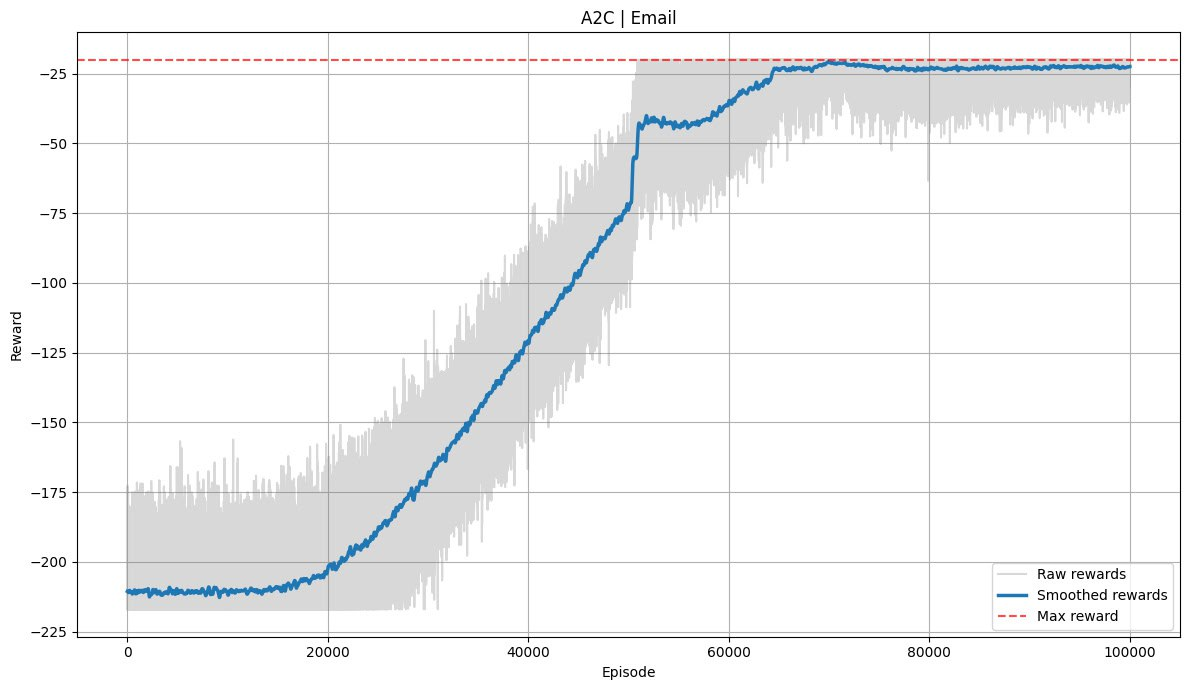
\includegraphics[width=0.7\textwidth]{./pictures/a2c_email.jpg}
  \caption[A2C convergence on Email Retrieval problem]
  {A2C convergence on Word Retrieval problem}\label{fig:a2c_email}
\end{figure}

\begin{figure}[H]
  \centering
  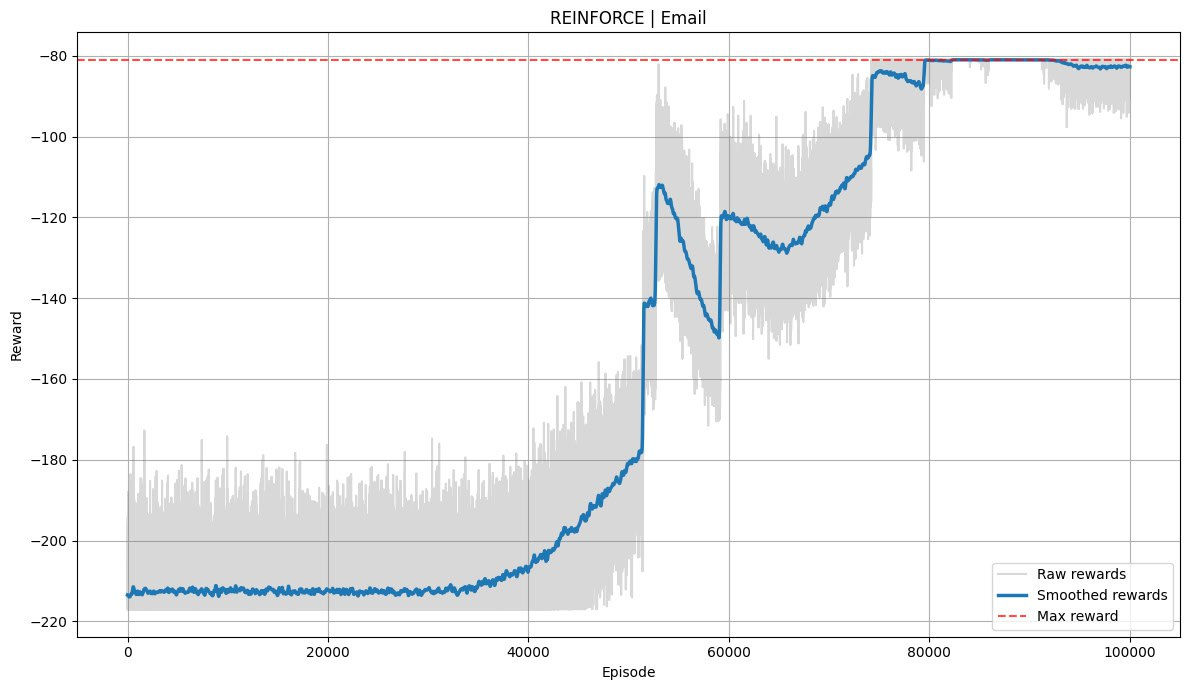
\includegraphics[width=0.7\textwidth]{./pictures/reinforce_email.jpg}
  \caption[REINFORCE convergence on Email Retrieval problem]
  {REINFORCE convergence on Word Retrieval problem}\label{fig:reinforce_email}
\end{figure}

\begin{figure}[H]
  \centering
  \begin{tabular}{l|l|l}
    \toprule
    \textbf{Agent} & \textbf{Achieved Regex} & \textbf{Total Reward} \\
    \midrule
    A2C            & \codeword{\w+@.*}       & -9430.51              \\
    REINFORCE      & \codeword{@.*}          & -40971.12             \\
    Random agent   & \codeword{Q:CnO<}       & -76470.91             \\
    \bottomrule
  \end{tabular}
  \caption{Final results for Email Retrieval problem. \textit{Total Reward} is the sum of rewards on all dataset samples}\label{tab:res_email}
\end{figure}

\paragraph{Dataset}
The dataset contains 500 strings of lengths from 11 to 35. Each string contains one email, which consists of 5 parts: from 4 to 8 letters, \codeword{@} sign, from 3 to 4 letters, dot, from 2 to 5 symbols.

\paragraph{Target regex}
We want our RL agent to simulate the application of \codeword{\w+@\w+\.\w+} regular expression.

\paragraph{Results}
\Cref{fig:a2c_email,fig:reinforce_email} show that both algorithms converged to some non-optimal
regular expressions. However, \Cref{tab:res_email} demonstrates that obtained regular expressions are more than reasonable though are not fully correct.


\section{Results and Discussion}

In this project our team successfully formulated regex generation as RL problem, implemented environment and tested several approaches Learning on our dataset, the some agents successfully learned how to get numbers and words consisting of certain letters. However, the agents cannot handle the formation of more complex expressions, for example, email extraction. While some of agents showed not the best performance, we proved, that such task can be indeed be solved via Reinforcement Learning.

% \begin{figure}[H]
%   \centering
%     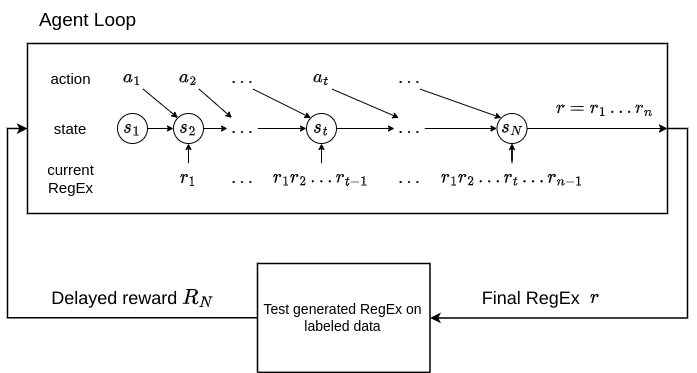
\includegraphics[width=0.5\textwidth]{./pictures/pipeline.png}
%     \caption[our pipeline]{our pipeline}\label{fig:pipeline}
% \end{figure}

% \begin{figure}[H]
%   \centering3\codetex{}
%     
\includegraphics[width=0.5\textwidth]{./pictures/rin.jpg}
%     \caption[zhopa]{zhopa}\label{fig:zhopa}
% \end{figure}

\bibliographystyle{plain}
\bibliography{references}

% \appendix
% % \section*{Appendix}


% \subsection*{Reinforce algorithm}
% \begin{algorithm}
%   \caption{Policy Gradient Training Loop}\label{algo:train_loop}
%   \begin{algorithmic}[0]
%     \Require{$\text{pgn\_net}:$ nn.Module, $\text{pgn\_optimizer}:$ optim.Optimizer, $\text{agent}:$ Agent, $\text{buffer}:$ TrajectoryBuffer, \\
%       \hspace{1em}$\text{epochs}, \text{episodes}:$ int, $\text{mean\_baseline}:$ bool, $\text{entropy\_beta}:$ float}
%     \State{$\text{arr\_rewards} \gets []$}
%     \State{$\text{pgn\_net.train()}$}
%     \For{$i \gets 1$ \textbf{to} $\text{epochs}$}
%     \State{$\text{buffer.clean()}$}
%     \State{$\text{state} \gets \text{env.reset()}$}
%     \State{$\text{done\_episodes} \gets 0$}
%     \State{$\text{ep\_states\_buf},\,\text{ep\_rew\_act\_buf},\,\text{reg\_exp},\,\text{train\_rewards} \gets [],[],[],[]$}
%     \While{$\text{done\_episodes} < \text{episodes}$}
%     \State{$\text{state\_tensor} \gets \text{Tensor}(\text{state})$}
%     \State{$\text{action\_logits} \gets \text{pgn\_net}(\text{state\_tensor})$}
%     \State{$t \gets 1 / \sqrt{i}$}
%     \State{$\text{action} \gets \text{agent.choose\_action}(\text{action\_logits} / t)$}
%     \State{$\text{next\_state},\,\text{reward},\,\text{done} \gets \text{env.step}(\text{action})$}
%     \State{$\text{reg\_exp.append}(\text{env.idx\_to\_action}(\text{action}))$}
%     \State{$\text{ep\_states\_buf.append}(\text{state});\quad \text{ep\_rew\_act\_buf.append}([\text{reward},\text{action}])$}
%     \State{$\text{state} \gets \text{next\_state}$}
%     \If{$\text{done}$}
%     \State{$\text{buffer.store}(\text{array}(\text{ep\_states\_buf}),\,\text{array}(\text{ep\_rew\_act\_buf}))$}
%     \State{$\text{ep\_states\_buf},\,\text{ep\_rew\_act\_buf} \gets [],[]$}
%     \State{$\text{train\_rewards.append}(\text{reward});\quad \text{arr\_rewards.append}(\text{train\_rewards})$}
%     \State{$\text{done\_episodes} \gets \text{done\_episodes} + 1$}
%     \EndIf
%     \EndWhile
%     \State{$\text{losses} \gets []$}
%     \ForAll{batch in $\text{buffer.get\_batches}(\text{mean\_baseline})$}
%     \State{$\text{pgn\_optimizer.zero\_grad}()$}
%     \State{$\text{state\_batch},\,\text{action\_batch},\,\text{reward\_batch} \gets \text{batch}$}
%     \State{$\text{logits\_v} \gets \text{pgn\_net}(\text{state\_batch})$}
%     \State{$\text{log\_prob\_v} \gets \text{LogSoftmax}(\text{logits\_v})$}
%     \State{$\text{log\_prob\_actions\_v} \gets \text{reward\_batch} \;\times\; \text{log\_prob\_v}[\dots,\;\text{action\_batch}]$}
%     \State{$\text{loss\_policy\_v} \gets -\,\mathrm{mean}(\text{log\_prob\_actions\_v})$}
%     \State{$\text{prob\_v} \gets \text{Softmax}(\text{logits\_v})$}
%     \State{$\text{entropy\_v} \gets -\,\mathrm{mean}\bigl(\sum(\text{prob\_v}\,\cdot\,\text{log\_prob\_v})\bigr)$}
%     \State{$\text{entropy\_loss\_v} \gets \text{entropy\_beta}\,\times\,\text{entropy\_v}$}
%     \State{$\text{loss\_v} \gets \text{loss\_policy\_v} - \text{entropy\_loss\_v}$}
%     \State{$\text{loss\_v.backward}();\quad \text{pgn\_optimizer.step}()$}
%     \State{$\text{losses.append}(\text{loss\_v})$}
%     \EndFor
%     \State{\textbf{print} epoch statistics}
%     \EndFor
%     \State\Return{$\text{arr\_rewards}$}
%   \end{algorithmic}
% \end{algorithm}

% \subsection*{Actor-Critic algorithm}

% \begin{algorithm}[H]

%   \caption{Actor-Critic}\label{algo:a2c}
%   \begin{algorithmic}[0]
%     \Require{empty state of size $n$, environment $env$}

%     \State{$done \gets False $}
%     \State{$actions \gets [] $}
%     \State{$states \gets [] $}
%     \State{$rewards \gets [] $}
%     \State{$state \gets env.reset() $}
%     \While{$!done$}
%     \State{$logits \gets net(state)[0]$}
%     \State{$action \gets choose\_action(logits)$}
%     \State{$new\_state, reward, done \gets env.step(action)$}
%     \State{$actions, states, rewards \gets action, state, reward$}
%     \EndWhile{}
%     \State{$cumulative\_rewards \gets accomulate(rewards)$}
%     \State{$logits, values \gets net(states)$}
%     \State{$loss\_val \gets MSE(values, cumulative\_rewards)$}
%     \State{$log\_probs \gets LogSoftmax(logits)$}
%     \State{$adv \gets cumulative\_rewards - values$}
%     \State{$log\_probs\_actions \gets adv \cdot log\_probs$}
%     \State{$loss\_policy \gets -mean(log\_probs\_actions)$}
%     \State{$probs \gets Softmax(logits)$}
%     \State{$entropy \gets mean(sum((probs \cdot log\_probs),dim=1))$}
%     \State{$entropy_loss \gets \beta \cdot entropy$}
%     \State{$loss\_policy.backward()$}
%     \State{$loss\_val \gets entropy_loss + loss\_val$}
%     \State{$loss\_val.backward()$}

%     \State{\Return{$net$}}

%   \end{algorithmic}
% \end{algorithm}


\end{document}